\section*{Neuroimaging}
Researchers who investigate the workings of the brain make use of a variety of specialised tools to extract different types of information. One dimension of information type concerns the spatial scale we consider. We can investigate at the microscale, the level of the individual neuron; or the macroscale, the level of thousands of neurons firing at the same time. But when we zoom in to the microscale, we can only measure a very small subset of the approximately 86 billion neurons in the human brain \cite{Herculano-Houzel2009}, and measurements on this scale utilise highly invasive procedures which are impractical for large-scale use in living humans. Macroscale procedures are less invasive and measure electric or magnetic fields outside the brain; through, for instance, electroencephalography (EEG) or magnetoencephalography (MEG). However, these procedures integrate signals from thousands of neurons and are difficult to spatially pinpoint with any precision. Another technique that can image the brain is MRI. While it does not measure neuronal activity directly, and is not as fast as M/EEG, it gives highly detailed three-dimensional images of the brain. MRI is not nearly specific enough for the microscale, but may just be able to pick up information from the organisational units that are formed by neurons: the cortical layers and cortical columns. In this thesis, we explore the possibility of using MRI for the mesoscale: the intermediate level between the neurons and the networks. We push the limits of fMRI analysis to prepare functional MRI (fMRI) for higher spatial resolution, so that we reach the level of the cortical layers (See Figure~\ref{fig:spatiotemporal}). This could teach us more about how neuronal networks communicate with each other and together accomplish the complex tasks of which the brain is capable.
\begin{figure}[H]
	\centering
	\includegraphics[width=0.8\textwidth, clip=true]{./Chapters/01_Introduction/Images/SpatioTemporalResolution}
	\caption{The temporal and spatial resolution of neuroimaging methods. By and large, methods of higher spatial resolution are more invasive. In this thesis, we tried to use the non-invasive technique of fMRI to cross the boundary of layer specificity. Picture recreated after Sejnowski et al. (2014) \cite{Sejnowski2014}.}
	\label{fig:spatiotemporal}
\end{figure}

\section*{Cortical layers}
The grey matter of the neocortex is a thin shell of approximately 3 mm \cite{Zilles1990} around the white matter. The white matter consists of long fibre tracts that relay signals from one brain area to another, but it is mainly in the grey matter that neuronal computations are performed. The grey matter itself consists of several shells: cortical layers (see Figure~\ref{fig:layers}) which are believed to have functionally distinct roles.
\begin{figure}[!ht]
	\centering
	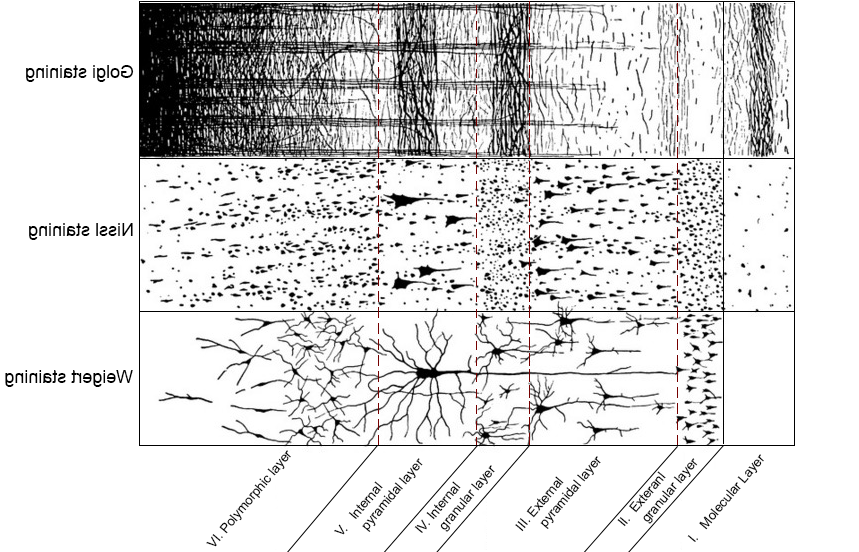
\includegraphics[width=0.8\textwidth, clip=true]{./Chapters/01_Introduction/Images/Layers}
	\caption{\cite{Brodman1909} }
	\label{fig:layers}
\end{figure}
In principle, ascending connections (feedforward, sensory; e.g., `I \emph{see} an apple') and descending connections (feedback, prediction; e.g., `I \emph{imagine seeing} an apple') are distinguished \cite{Rockland1979} and can be related to hierarchical ranks of processing \cite{Barone2000}. A given node in the cortical hierarchy will receive feedforward input that targets layer 4 and to a lesser extent layer 5 \cite{Constantinople2013}. These predominantly originate from supragranular layers (see Figure~\ref{fig:layerprocessing}). On the other hand, feedback connections from higher areas terminate primarily in layers 1 and 5, but avoid layer 4 \cite{Anderson2009}. The differential contribution of feedforward and feedback activation is not well established \cite{Shipp2013}. This `canonical microcircuit' describes the excitatory relay of information within the cortex. While the specifics of the performed computations are largely unknown, in general the two types of information can be somewhat speculatively linked to the predictive coding framework \cite{Friston2010}. This framework states that at the fundamental level, the brain continuously receives predictions from higher regions (feedback signal) which it compares to \emph{prediction error} from lower regions (feedforward signal). Based on this comparison, it makes new predictions and prediction errors and thus continues in a recurrent process of updating knowledge based on new information. Through this link to the predictive coding framework, the cortical layers can provide a more mechanistic understanding of the computations in the brain \cite{Shipp2016}.
\begin{figure}[!ht]
	\centering
	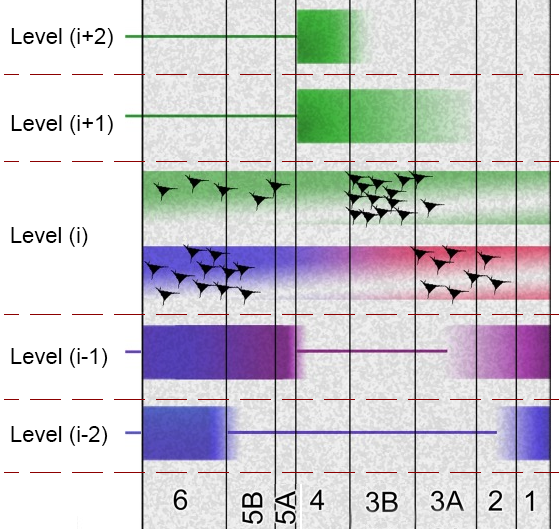
\includegraphics[width=0.5\textwidth, clip=true]{./Chapters/01_Introduction/Images/LaminarProcessing}
	\caption{Layer specific processing, adapted from Ship et al. (2013)\cite{Shipp2013}. From region $i$, there are feed forward connections (green) primarily targeting the middle layers in region higher in the cortical hierarchy ($i+1, i+2, \ell$). Feedback connections (blue, purple) target top and deep layers in lower regions in the hierarchy ($i-1, i-2, \ell$).}
	\label{fig:layerprocessing}
\end{figure}

The layers can be used to learn about information processing within a single region, but neurons also form connections with more distant regions, affording us the potential means to investigate laminar specific, cross-regional communication. Tracer studies reveal large networks of regions via feedforward and feedback connections \cite{Felleman1991}, see Figure~\ref{fig:felleman}. Tracers heavily rely on (post-mortem) structural connectivity, so even though the connections themselves can be mapped out, the strength and nature of the connections remain unclear. This is why \emph{in vivo} investigation of the cortical layers could add new information to the workings of directional and causal communication during task performance. Current work into interregional causal inference in the brain primarily relies on characteristics of haemodynamic consequences of brain interaction in Dynamic Causal Modelling (DCM) \cite{Friston2009} or timing differences in signals with Granger Causality \cite{Aalen2007}, which can further be used to establish cortical hierarchies \cite{Michalareas2016}. The cortical layers may provide complementary information on interregional feedforward and feedback communication in living subjects and could tell us more about the crosstalk between regions at the network level.
\begin{figure}[!ht]
	\centering
	\includegraphics[width=0.6\textwidth, clip=true]{./Chapters/01_Introduction/Images/Felleman}
	\caption{Picture adapted from Felleman \& Van Essen (1991) \cite{Felleman1991}. A graphical depiction of cortical regions with structural connections as obtained by post-mortem tracer studies. This is also a rudimentary reflection of hierarchical processing in the brain. As these connections originate from and target specific layers, it would be interesting to see if similarities can be found in the layer specific fMRI signal. This could allow for making hierarchical statements about neuronal processes based on fMRI data.}
	\label{fig:felleman}
\end{figure}

Across cortical regions and across species, the layered structure of the cortex is largely conserved. It is therefore likely that many of the computational underpinnings translate from one brain region to the next \cite{Buonomano1998}. Thus, a better understanding of layer specific processing in specific regions and during specific tasks could teach us more general principles of brain organisation. One can imagine that for some perceptual tasks, feedforward drive may dominate the computation, for example when a lot of sensory input is involved. Alternatively, when strong predictions, expectations, or imagination is involved, feedback will likely play a larger role. Linking the basic feedforward and feedback information pathways to conceptual level cognitive domains such as language, memory, or emotion is a difficult task for the future. To obtain a better mechanistic understanding of these evolutionary achievements, it is important to learn more about laminar processing.

There is a variety of cognitive functions for which layer specific dissociation could already be an interesting tool, as there are clear predictions with respect to feedback and feedforward drive \cite{Lawrence2017}. For example, in the area of visual attention, prediction, or saliency, it could be interesting to compare and contrast the different types of hypothesised feedback drive against visual feedforward drive. Layer specific dissociation may also be useful in clinical applications, as some mental disorders are expected to have abnormalities in directional communication between brain regions. Hallucinations and delusions are strongly linked to abnormal perception and are hypothesised to have different predictive coding mechanisms \cite{Fletcher2008}. This may well be reflected in neurophysiological traces of the cortical layer activation patterns.

Interesting similarities with the brain are found in the emerging field of deep learning networks. Convolutional layers of the networks have been correlated to the visual hierarchy of the brain \cite{Guclu2015}, and it would be interesting to look for similarities at an even deeper level. Given that deep learning networks work with feedback and feedforward propagation of signals, it could also be interesting to relate their features to the cortical layers.

Therefore, signals from the cortical layers in a brain region may contain information about the nature of computations and about communication with other regions. Investigating this during task performance could open doors to new types of information and shed light on a multitude of cognitive processes. However, the greatest barrier is that the layers (and neuronal communication in general) are not easily measured. The most realistic current measurement technique is functional Magnetic Resonance Imaging, due to its high spatial resolution and non-invasiveness. Unfortunately, fMRI does not measure neuronal firing directly, but only picks up changes in blood oxygenation that occur as a result of neuronal firing. We therefore first need to gain a better understanding of what type of information it is that fMRI gives us.

\section*{MRI}
The basis of magnetic resonance imaging (MRI) is the phenomenon of nuclear magnetic resonance (NMR). In principle, this describes the magnetic behaviour of protons and neutrons in terms of their \emph{quantum spin}: a preferred axis of rotation of an elementary particle. Normally, each spin has a random orientation of the axis of rotation. In the presence of a magnetic field, however, the spins will start precessing around the axis of the main magnetic field. The speed of rotation (angular frequency) will be directly proportional to the magnitude of the field: the Larmor frequency. In 1946, Felix Bloch and Edward Purcell independently performed the first experiments in which they manipulated the spins with radio frequency (RF) pulses, for which they later received a Nobel prize. Bloch described the nuclear magnetisation of a material as a function of its relaxation times $T_1$ and $T_2$ \cite{Bloch1946}. The $T_1$ value describes the time it takes for longitudinal magnetisation (aligned with the magnetic field) in a certain material to return to thermal equilibrium after it has been excited by an RF pulse. The $T_2$ value describes the time constant with which the transverse magnetisation (perpendicular to the magnetic field) decays as a result of loss of the phase coherence between spins. Further development of the measurement technique by Paul C. Lauterbur in 1973 \cite{Lauterbur1973}, for which he received a Nobel prize thirty years later, allowed for the measurement of these properties as a function of two-dimensional space. Initially, the approach was much like the tomographic back-projection technique that forms the basis of Computed Tomography (CT). This description formed the basis of gradient echo imaging, where an applied magnetic field (gradient), additional to the main magnetic field, gives rise to a signal from which an image can be reconstructed. A later description was a formalism in which the spatial frequencies of an image, $k$-space, is described as an integral of the gradient \cite{Twieg1983,Ljunggren1983}:
\begin{equation}
\vec{k}(t)=\gamma \int_{0}^{t}\vec{G}(t')dt'
\end{equation}
This is still the basis of current MR imaging. The equation represents the mapping of spatial frequencies in an image as a function of the applied gradient over time. The original simple graphical representation is shown in Figure~\ref{fig:kspace}. If the gradients are applied so that a large part of $k$-space is homogeneously covered, the spatial frequencies are accurately sampled. The $k$-space signal is the Fourier transform of the spin density distribution $\rho (\vec{r})$,
\begin{equation}
S(t)=\hat{\rho}(\vec{k}(t))=\int\rho(\vec{r})e^{i \vec{k}(t) \cdot \vec{r}}d\vec{r},
\end{equation}
so that the $k$-space can easily be transformed into an image of the spin density.
\begin{figure}[!ht]
	\centering
	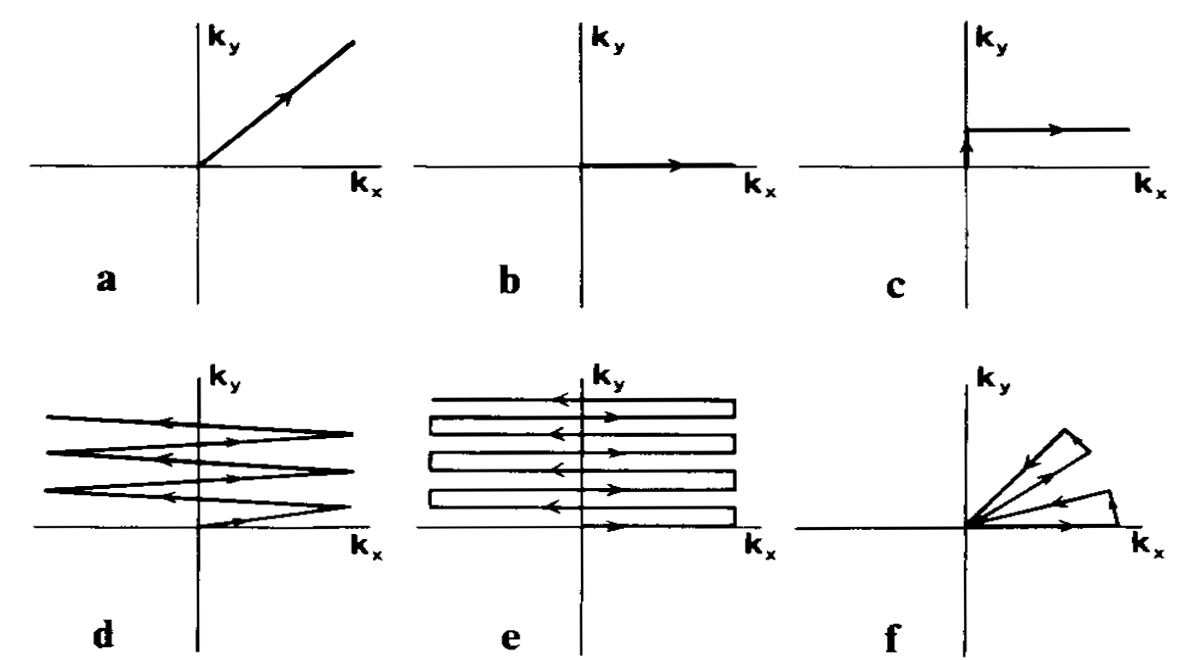
\includegraphics[width=0.6\textwidth, clip=true]{./Chapters/01_Introduction/Images/Kspace}
	\caption{ \cite{Ljunggren1983}. }
	\label{fig:kspace}
\end{figure}

The aforementioned $T_1$ and $T_2$ mechanisms occur as the result of random processes of spins returning to equilibrium. There is an additional mechanism, $T_2^*$, in which the dephasing of the spins is not random but predictable, and thus reversible. After an RF pulse, spins start out by pointing in the same direction, but then fan out and start to systematically dephase in clockwise or counter-clockwise direction. Hence, the spins will cancel each other out, so that the signal decays much faster than $T_2$, but instead with $T_2^*$. However, the accumulated phase can be reversed (by a 180\textdegree~RF pulse), so that they start to converge until they point in the same direction again to form a \emph{spin echo}. As a result, gradient echo images are $T_2^*$-weighted and spin echo images are $T_2$-weighted.

\section*{Contrast Mechanisms}
So, MRI scanners can be used to obtain a variety of types of information, but is any of it relevant to the study of cortical layers? At the core, all contrasts are results of changes in magnetic properties. All materials have a magnetic \emph{susceptibility}: the extent to which they become magnetised by an external magnetic field. If the material resists the magnetic field (i.e., negative susceptibility) it is diamagnetic, and if it assists the field (i.e., positive susceptibility) it is paramagnetic. Certain metals (e.g., iron, nickel, cobalt) have very high susceptibility and are called ferromagnetic. These are the materials that are commonly attracted by standard refrigerator magnets. Red blood cells contain haemoglobin, which is paramagnetic when it does not carry oxygen (deoxyhaemoglobin) because of the high spin state of the iron atom \cite{Pauling1936}. The change in magnetic susceptibility of red blood cells when they are oxygen rich or oxygen poor is called the Blood Oxygenation Level Dependent Signal: the BOLD signal \cite{Ogawa1990}. So, while neuronal firing does not change magnetic properties directly, synaptic activity indirectly causes changes in blood flow that may be picked up with an MRI scanner \cite{Logothetis2001}. It is of note that large parts of the biological mechanisms behind the neurovascular relationship are still disputed; most importantly, the extent to which the BOLD response reflects laminar specific activation is largely unknown.

Fundamentally, the BOLD signal arises as a consequence of magnetic field perturbations arising from deoxyhaemoglobin molecules \cite{Norris2006}. These changes extend beyond the blood vessel into the tissue and depend on field strength, the orientation of the vessel, and the vessel diameter, as well as the concentration of deoxyhaemoglobin. From the time that the molecules are excited until the time of the echo, molecules in the tissue move around the vasculature. If the trajectory of a molecule in this time is small compared to the vessel size (and hence compared to the drop-off), there is little change in its local magnetic field and the phase accumulation is reversible: a static effect. If, on the other hand, the molecule's trajectory is large, it will stochastically sample the local field, leading to random and hence irreversible phase changes. These two contrast mechanisms are the static and dynamic extravascular dephasing effects. The magnetic field perturbations around the vessels scale linearly with field strength. It is thus not surprising that the static effect also increases linearly with field strength, however, as the dynamic effect arises from diffusion-based attenuation, it increases quadratically.  At high field strengths, the dynamic effect is sensitive to small vessels and  and thus very specific to the origin of the activation, but detecting it requires high sensitivity \cite{Panchuelo2014}. At the same time, the static effect results in high activation from venous vessels and may in part be detected further downstream from the site of activation. 

An additional source of BOLD contrast is the intravascular effect. The magnetic field inside the vessel is slightly different from the surrounding tissue because of the amount of deoxyhaemoglobin. As a result, the signal will start to dephase with respect to the extravascular signal. This effect can be reversed because it is constant over time; it is called the static intravascular effect. 

The last contrast mechanism that contributes to the BOLD signal is disputed in origin. This is irreversible (dynamic) intravascular dephasing and has to do with the random movement of water molecules in blood vessels. It can be viewed as either caused by exchange with a deoxyhaemoglobin molecule's paramagnetic centre, or in terms of diffusion around the blood cells, but no experiment to date has been able to tease the two mechanisms apart. The intravascular effects will accumulate in downstream vessels,  and are thus less specific.

Given the four BOLD contrast mechanisms, there is still an outstanding question about the proportions they each contribute in measurements. This may even vary at the laminar level, as the deoxyhaemoglobin from deeper layers flows upward to the higher layers. The relative contributions of the contrast mechanisms in combination with the blood flow effect have been modelled for both spin echo and gradient echo: the results suggest that most of the signal produced in a layer is also visible in that layer \cite{Markuerkiaga2016,Uludag2017}. For spin echo the flow effect is minimal; gradient echo has a tail that extends to more superficial layers, but also has a higher sensitivity.

The 180\textdegree~pulses in spin echo experiments reverse all static effects. Therefore, spin echo is only sensitive to the ($T_2$-weighted) dynamic contrast mechanisms and is less sensitive than gradient echo, to which all four mechanisms contribute. At higher field, the contribution of the intravascular effect is significantly smaller because of the shorter $T_2$-value of blood \cite{Norris2006}. Thus, spin echo at high field is heavily weighted to the extravascular dynamic effect, which theoretically makes it well suited to laminar fMRI. Unfortunately, it is harder to run spin echo sequences at higher fields, as the number of 180\textdegree~pulses increases the specific absorption rate to the extent that this limits its application. Therefore, both spin echo and gradient echo have advantages and disadvantages. A range of laminar profiles has been found using spin echo (e.g., \cite{Zhao2004,Harel2006,Goense2006}) and gradient echo (e.g., \cite{Polimeni2010,DeMartino2013,Chen2013}). A combination of both has also been tried: GRadient A Spin Echo (GRASE) \cite{Olman2012,DeMartino2013}.

A different contrast is that of Arterial Spin Labelling (ASL) \cite{Williams1992,Detre1994} that measures cerebral blood flow (CBF). CBF varies in a laminar specific fashion \cite{Gerrits2000} and may be measured with ASL at the submillimetre level \cite{Ivanov2016}. There are many variations of ASL, but for clinical application the field has reached consensus on a preferred implementation \cite{Alsop2015}. At the core, blood is `labelled' by means of an RF pulse. The labelled blood has different magnetisation and travels downstream where it crosses the capillary bed and enters the tissue. After a post-labelling delay (PLD), the blood has moved out of the arterioles, but to adequately measure tissue perfusion, PLDs can be over a second. The labelled image is only interpretable when it is compared to a similar control image \emph{without} the labelling, but with otherwise completely equivalent contrast. This way, theoretically, the subtraction removes all signal from the stationary tissue, and only the difference due to the inflow of blood remains to form perfusion images of the brain \cite{Petcharunpaisan2010}. Oftentimes, additional RF pulses are applied to further reduce background tissue signal \cite{Garcia2005,Grade2015}. Because of the large PLD and the fact that it requires two images, ASL is an inefficient process, which probably makes the technique unsuitable for laminar fMRI.

Next to cerebral blood \emph{flow}, one can also look at cerebral blood \emph{volume}. Blood vessels may dilate and contract as a function of the activity of a brain region. This can be measured with Vascular Space Occupancy (VASO) \cite{Lu2003} and can reveal layer specific differences \cite{Zhao2006,Huber2018}. VASO makes use of the fact that the $T_1$ values of arterial and venous blood are very close together and both are a lot longer than the $T_1$ of tissue. By inverting all signal and measuring at an inversion time where the blood signal goes through zero, the only signal that is left has to come from tissue. Effectively, the remaining signal represents the contribution of tissue in a voxel. On neuronal activation, blood vessels expand and increase in voxel contribution, which decreases the tissue contribution and lowers the signal. Thus, the VASO signal decreases on activation. At higher field strengths, the $T_1$ values of tissue and blood are closer together, which makes it harder to get a VASO contrast. Much work has been invested to make VASO work in human fMRI for 7 Tesla, and it indeed shows task dependent layer specific differences \cite{Huber2017}.

Figure~\ref{fig:microvasulature} shows the microvasculature of a small piece of visual cortex in a macaque. Shown in red are the arterioles: small blood vessels that dive from the top of the cortex (the pial surface) downward to supply the whole grey matter with blood. The smallest vessels, the capillaries, relay the oxygen to the neurons in all cortical layers, so that deoxygenated haemoglobin is drained away by the veins (blue). The veins on top of the cortex, which can be an order of magnitude larger than the cortical veins, accumulate and carry off the deoxygenated blood. From this, one can appreciate the difficulty of extracting laminar specific signals with large signals of non-interest in the direct neighbourhood.
\begin{figure}[!ht]
	\centering
	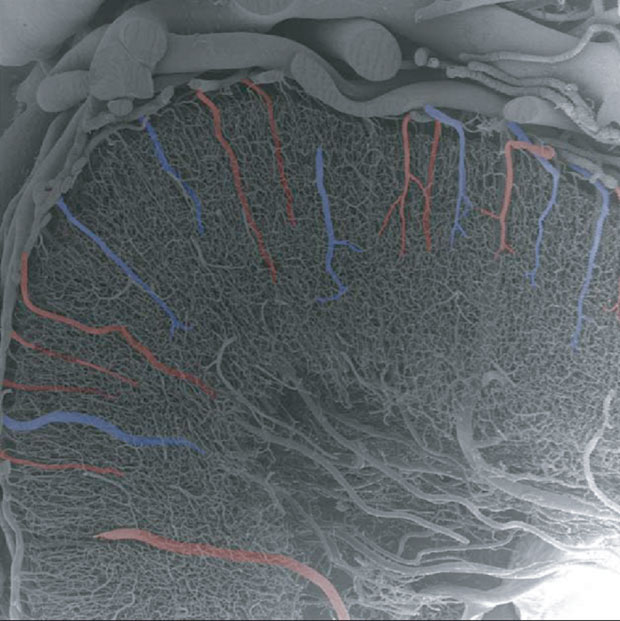
\includegraphics[width=0.9\textwidth, clip=true]{./Chapters/01_Introduction/Images/Microvasculature}
	\caption{The microvasculature of the visual cortex of a macaque \cite{Weber2008}. }
	\label{fig:microvasulature}
\end{figure}

The level of measured blood oxygenation depends on several factors. On activation, more blood starts flowing (higher cerebral blood flow (CBF)), vessels start dilating (greater cerebral blood volume (CBV)), and the consumption of oxygen increases (higher cerebral metabolic rate of oxygen (CMRO$_{2}$)). These quantitative measures can be related to one another, save for some free parameters that need to be empirically determined \cite{Davis1997}. However, although the proposed equations hold for the cortical column in its entirety, they do not take into account potential layer specific differences. So, we cannot directly measure neuronal activation with MRI: the closest we can get is the traces in magnetic properties in the vasculature through BOLD, CBV, CBF, and CMRO$_{2}$. The extent to which these quantities vary at spatially specific levels of the cortical layers is an outstanding question, however, and needs to be empirically tested. Indeed, there are techniques to measure them: $T_2^*$-weighted imaging for BOLD \cite{Norris2006}, VASO for CBV \cite{Huber2018}, arterial spin labelling for CBV \cite{Grade2015}, and calibrated BOLD for CMRO$_{2}$ \cite{Blockley2013}. All these vary in terms of sensitivity, specificity, and attainable resolution (spatial as well as temporal). The spatial resolution, in combination with the type of experiment that is required, makes CBF and CMRO$_2$ measurements poor candidates for human \emph{in vivo} fMRI. It is mainly BOLD and CBV that have shown promising layer specific differences in animal experiments \cite{Lu2004,Zhao2006,Jin2008,Goense2012}. The main benefits of VASO compared to BOLD are its quantifiability \cite{Lu2003} and local specificity \cite{Jin2006}, whereas BOLD has higher sensitivity and speed \cite{Huber2018}.

\section*{Acquisition}
We have seen that MRI can be used to measure different magnetic properties, potentially in combination with physical and physiological properties of the brain. For our purposes, we are interested mainly in the properties of the BOLD response, which we use to rapidly create images of the brain. Every few seconds, an image is acquired that is a reflection of the BOLD response at that moment. We would like to have as many images as possible as we aim to measure real-time responses to our experiments. As a result, we may have to make compromises in the spatial resolution, signal-to-noise ratio, or contrast-to-noise ratio. Functional ($T_2^*$-weighted) images are optimal for measuring BOLD activity, but do not show a particularly clear differentiation between the white matter and the grey matter (see Figure~\ref{fig:mybrain}). For accurately distinguishing the cortical layers, another image is required, with better anatomical contrast. For this, a structural (or anatomical) scan is used. It cannot be acquired in several seconds, as is the case with the functional scan; instead it takes several minutes. Typically, a structural scan is $T_1$-weighted and shows high anatomical contrast because the $T_1$-value of the myelinated white matter is shorter than the $T_1$-value of the grey matter \cite{Wansapura1999}. It is often sufficient to compute a cortical reconstruction: a three-dimensional representation of the cortical surface. A cortical reconstruction can be a useful way of looking at the brain as a geometrical shape and can facilitate a variety of subsequent analyses.
\begin{figure}[!ht]
	\centering
	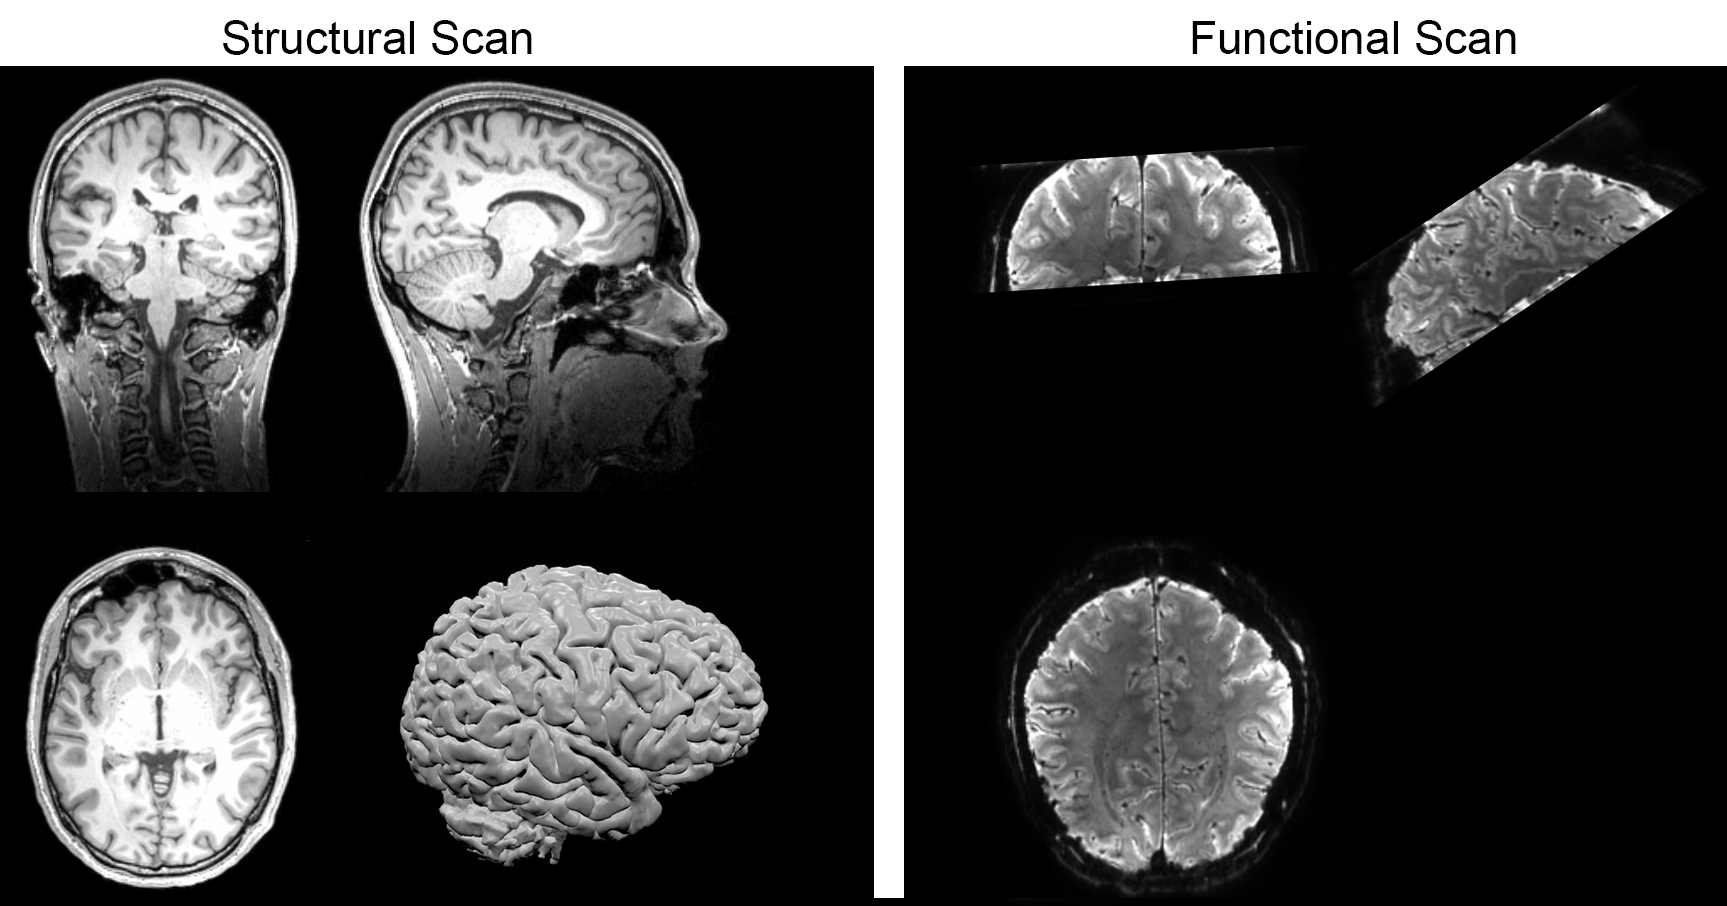
\includegraphics[width=0.99\textwidth, clip=true]{./Chapters/01_Introduction/Images/MyBrain}
	\caption{An example of a structural and functional brain scan. On the left, the structural scan has high anatomical contrast and sharp differences between the white matter and grey matter. The contrast is sharp enough to make a three dimensional reconstruction of the brain (lower right corner). On the right, a functional image is shown. The anatomical contrast is much weaker, but it can be acquired quickly and the contrast is susceptible to slight changes in blood deoxyhemoglobin, related to oxygen consumption on neuronal activation.}
	\label{fig:mybrain}
\end{figure}

Much research has been done to retrieve new types of information with MRI. Complementary to this, improving the speed of the acquisition has always been an important point of development. There is a variety of ways in which this can be done. Acceleration techniques can make use of the mathematical properties of the acquired signal (Hermitian symmetry of the $k$-space), in order to acquire only a part of the $k$-space in partial Fourier acquisitions \cite{Feinberg1986}. Alternatively, information can be added to the reconstruction equations by adding in information about the sensitivity of receiver coils. Techniques like GRAPPA, SENSE, and CAIPIRINHA use this type of information, which can make the acquisition several times faster \cite{Setsompop2016}. In general, MRI data contains several forms of spatiotemporal redundancy that can be exploited to speed up the acquisition \cite{Tsao2012}. Using these techniques is essential for increasing the spatial resolution, temporal resolution, or the signal-to-noise ratio per volume.

The acquisition of anatomical scans is relatively straightforward as there is no pressure to acquire a volume every several seconds. One can rely on standard acquisition protocols for MPRAGE sequences \cite{Mugler1990} or use a version that is less susceptible to intensity biases but that takes longer to acquire, the MP2RAGE \cite{Marques2010}. For functional images, there are more constraints and parameters to consider, out of which we will here discuss the difference between 2D and 3D acquisitions. A three-dimensional MRI volume can be acquired in several ways. In a 2D acquisition, a stack of slices is sequentially acquired and put on top of each other. This requires excitation of a single slice at a time, and the two-dimensional encoding of each plane. For each plane, the $k$-space (all spatial frequencies) is sampled and converted to an image by means of a Fourier transform. This makes for a smooth planar image, but as the stack of images is scanned sequentially, the vertical transition ($z$-direction) may be less smooth. Every movement of the brain during the acquisition will result in images not precisely landing on top of each other, so that images may show a `staircase artefact' in the vertical direction. The higher the resolution, the more pronounced this staircase artefact will be. In addition, towards higher resolution the two-dimensional excited slabs need to become smaller, which requires a sharper slice profile. This in turn requires longer pulses that easily cause higher specific absorption rates and may cause peripheral nerve stimulation. Many of these factors can be circumvented with a 3D acquisition \cite{Poser2010}. Instead of a plane-by-plane excitation and read-out, the entire volume is excited \cite{Song1994} to fill a three-dimensional $k$-space. The image can then be reconstructed by a single three-dimensional Fourier transform instead of a series of two-dimensional Fourier transforms. This way, transitions between slices are smoother, which is important for cortical layering. As a downside, any movement during the acquisition will cause noise (blurring) in the entire image, so 3D imaging is more vulnerable to physiological effects. However, this is generally outweighed by the shorter volume TR that can more easily be achieved by acceleration techniques \cite{Poser2010}. Because there is no limitation of slice-by-slice acquisition in the $z$-direction, this dimension can be used for parallel imaging. At high spatial resolution, 3D imaging is faster and has a higher sensitivity.

Choosing a sequence requires carefully balancing the advantages and disadvantages against each other. Here, for its higher sensitivity, we chose to use gradient echo with a 3D EPI acquisition to investigate the laminar BOLD signal, at a field strength of 7 Tesla for high specificity. The potential downside of this is the susceptibility to the larger veins on top of the cortex that might obscure smaller effects \cite{Barth2007}.

\section*{FMRI analysis}
After covering the fundamentals of measurement techniques, it is clear what types of information may be expected to be present in the data. Extracting the relevant information, however, is at least as complicated as the data acquisition. The brain is a highly convoluted structure, which we are trying to describe and visualise by means of cubic voxel rasters. The first problem we encounter is a geometrical one: how do we attach a brain location to voxels in space? This can be done by making a \emph{cortical reconstruction} on a high-resolution brain scan \cite{Dale1999,Bazin2012}, with a very clear contrast between the white matter and grey matter as seen in Figure~\ref{fig:mybrain}. The distinction between white and grey matter is clear enough to draw a three-dimensional boundary on both sides of the grey matter: on the white matter boundary and on the pial surface, the separation between the grey matter and the cerebrospinal fluid (CSF).

The cortical reconstruction is informative about the shape of the brain and potentially also about the layers: one could imagine different layers as intermediate surfaces between both outer boundaries, the locations of which could then be used to sample the cortical layers \cite{Koopmans2011,Polimeni2010,DeMartino2013}. This description allows for a multitude of surface-based calculations \cite{Fischl2000,Bazin2012} and, for example, can serve as the basis for an anatomically motivated parcellation of the cortex  \cite{Bok1929,Waehnert2014}. Along the many curves of the cortex, cytoarchitectonic layers approximately conserve volume in a given cortical column. Taking a more naturalistic flow of the cortex into account can provide a clear advantage in high-resolution laminar analysis \cite{Waehnert2014}.

The cortical reconstruction can be made on a dedicated high-resolution high-contrast scan, but this does not yet give functional information. First, the cortical surfaces need to be `coregistered' with the functional data and brought into the same analysis space. Unfortunately, this is made considerably more difficult by two main factors. First, the contrast and resolution of standard gradient echo functional data are poor, so there is not a lot of information on which to base a good coregistration. Secondly, when `echo planar imaging' (EPI) is used, a fast acquisition scheme to collect data, the data will to some extent be geometrically distorted. The reason is that the scanner magnetic field is not everywhere exactly equal. When we talk about a scanner with a field strength of 7 Tesla, this means there should be a stable static magnetic field of that strength in the centre of the scanner. However, because the presence of a human body perturbs the field, in practice it is not as homogeneous as one might desire. Small perturbations can be corrected by \emph{shimming}: applying an additional magnetic field to compensate for the inhomogeneities. However, this is not accurate enough to correct all deviations and the inhomogeneities need not even be constant over time. As mentioned before, MRI is based on spins precessing at a frequency that is proportional to the field strength. By adding an additional linear magnetic field gradient, the frequency of the spins essentially encodes their spatial locations.  When a local inhomogeneity is present in the volume, in effect the spins precess faster or slower than assumed, and as a result they are displaced in the image. Since the displacement is field strength dependent, distortions are more pronounced at higher fields. These can easily be of the order of several millimetres, which comes down to a shift of the size of the entire cortex. Therefore, extreme care must be taken in aligning scans properly and thoroughly checking the correctness of the cortical surface in the regions that one wants to analyse. The severity of distortions is directly dependent on the bandwidth per pixel and field strength \cite{Jezzard1995,Schmitt1998}. In the phase encoding direction, the bandwidth is a lot lower in an EPI acquisition. Given that $k$-space is acquired in a standard raster pattern, for every line in the frequency direction, one goes up only a single point in the phase encoding direction. As a result, the distortions in the phase encoding direction can easily be two orders of magnitude larger than in the frequency direction.

There is a wide variety of other potential noise sources that can contaminate the (laminar) signal. Participants in a study will move several millimetres, breathe, and have a heartbeat that is clearly visible in the signal. During an experiment, people may suffer lapses in attention, hypnagogic episodes, and so on. Many operations are performed on the data to remove as many sources of noise as possible; this creates long analysis pipelines. This makes the process of doing fMRI analysis difficult at the conceptual level, and may also create a logistical nightmare: different software packages, programming languages, data types, data representations, and different styles of programming. As a result, it is understandable that the reproducibility of fMRI results can be low \cite{Nosek2015,Gorgolewski2016a}. Here we took care to build and use all tools as reproducibly as possible and to provide all data openly, accompanied by the scripts to generate the results.

\section*{Laminar Analysis in Human FMRI}
A lot of information about the computations in the brain may be uncovered through better understanding the cortical layers. Invasive electrophysiological recordings have indeed found relevant laminar differentiation in macaques \cite{Buffalo2011,Maier2010,Maier2011,VanKerkoerle2017}, and while the exact origins of the BOLD signal are still unknown, there is strong evidence that the BOLD signal has a laminar footprint \cite{Goense2006}. This is confirmed by Yu et al. \cite{Yu2014}, where they show clear layer specificity in the onset of the BOLD response, but no prolonged laminar differentiation that could be picked up with the temporal resolution of conventional human fMRI. While it is known which layers are initially targeted by feedback and feedforward signals, little is known about their further processing. There is evidence that excitatory neurons may quickly redistribute input from the thalamus by means of their local axonal collaterals \cite{Guy2017,ReyesPuerta2015}. As a result, cortical activity may nearly instantaneously spread over several layers and columns, to the detriment of the laminar specificity of the BOLD signal.

The field of laminar analysis is still in its infancy, but there is a growing body of work that claims to have found hypothesised laminar differentiation in humans \cite{Maass2014,Muckli2015,Scheeringa2016,Kok2016,Huber2017}. Unfortunately, all of these studies use different methods for largely the same type of analysis. To date, no published replications exist of layer specific human \emph{in vivo} studies that could reinforce these findings. With the variations in analysis, many uncertainties in the data, and the small size of the potential effect, it is clear that any potential effect can only be picked up with powerful methods that address as many sources of noise as possible. In this thesis, we constructed a robust and reusable analysis pipeline in which we solved key issues in laminar analysis; thereby we envision making laminar specific investigations a more routine type of study.

